\section{Extraction of the G Double-Polarization Observable}
The Cross section for this reaction, considering the target linear Polarization along the photon beam direction $P_z$, and the Polarization of the photon beam ($P_{\parallel}$ (Electric field parallel to the floor) and $P_{\perp}$ (Electric field perpendicular to the floor)), can be written as:
\begin{equation}
\frac{d\sigma}{d\Omega} = \left(\frac{d\sigma}{d\Omega}\right)_{UNPOL}  \left( 1 + P_{\gamma}cos(2\phi) + P_{\gamma} P_z sin(2\phi) \right)
\end{equation}

During the g9a run period all the possible combinations of different polarizations where measured, reaching the full configuration

\begin{eqnarray}
\left(\frac{d\sigma}{d\Omega}\right)_{\parallel +} = \left(\frac{d\sigma}{d\Omega}\right)_{UNPOL}  \left( 1 + P_{\gamma \parallel}cos(2\phi) + P_{\gamma \parallel} P_z sin(2\phi) \right) \\
\left(\frac{d\sigma}{d\Omega}\right)_{\parallel -} = \left(\frac{d\sigma}{d\Omega}\right)_{UNPOL}  \left( 1 + P_{\gamma \parallel}cos(2\phi) - P_{\gamma \parallel} P_z sin(2\phi) \right) \\
\left(\frac{d\sigma}{d\Omega}\right)_{\perp +} = \left(\frac{d\sigma}{d\Omega}\right)_{UNPOL}  \left( 1 + P_{\gamma \perp}cos(2\phi) + P_{\gamma \perp} P_z sin(2\phi) \right) \\
\left(\frac{d\sigma}{d\Omega}\right)_{\perp -} = \left(\frac{d\sigma}{d\Omega}\right)_{UNPOL}  \left( 1 + P_{\gamma \perp}cos(2\phi) - P_{\gamma \perp} P_z sin(2\phi) \right)
\end{eqnarray}
An asymmetry between these configurations will permit to extract the desired parameter $G$. In order to normalize these measurement before calculating the asymmetry, the cross section was also calculated with the same configurations for the Polarized target, but with an amorphous crystal (Carbon), in order to create an unpolirized photon beam. This will also remove effects due to the acceptance of the detector. 

\subsection{Calculation of the flux on target, F}
During the experiment, every effort was made to collect the same amount of data for all four possible combinations of polarised beam-polarised target settings. In practice, however, the flux incident on the target for the PARA and PERP beam settings was not equal and the $\pi^+$ azimuthal distributions had to be scaled to each other before any further analysis.
\begin{figure}[htb]
  \begin{center}
    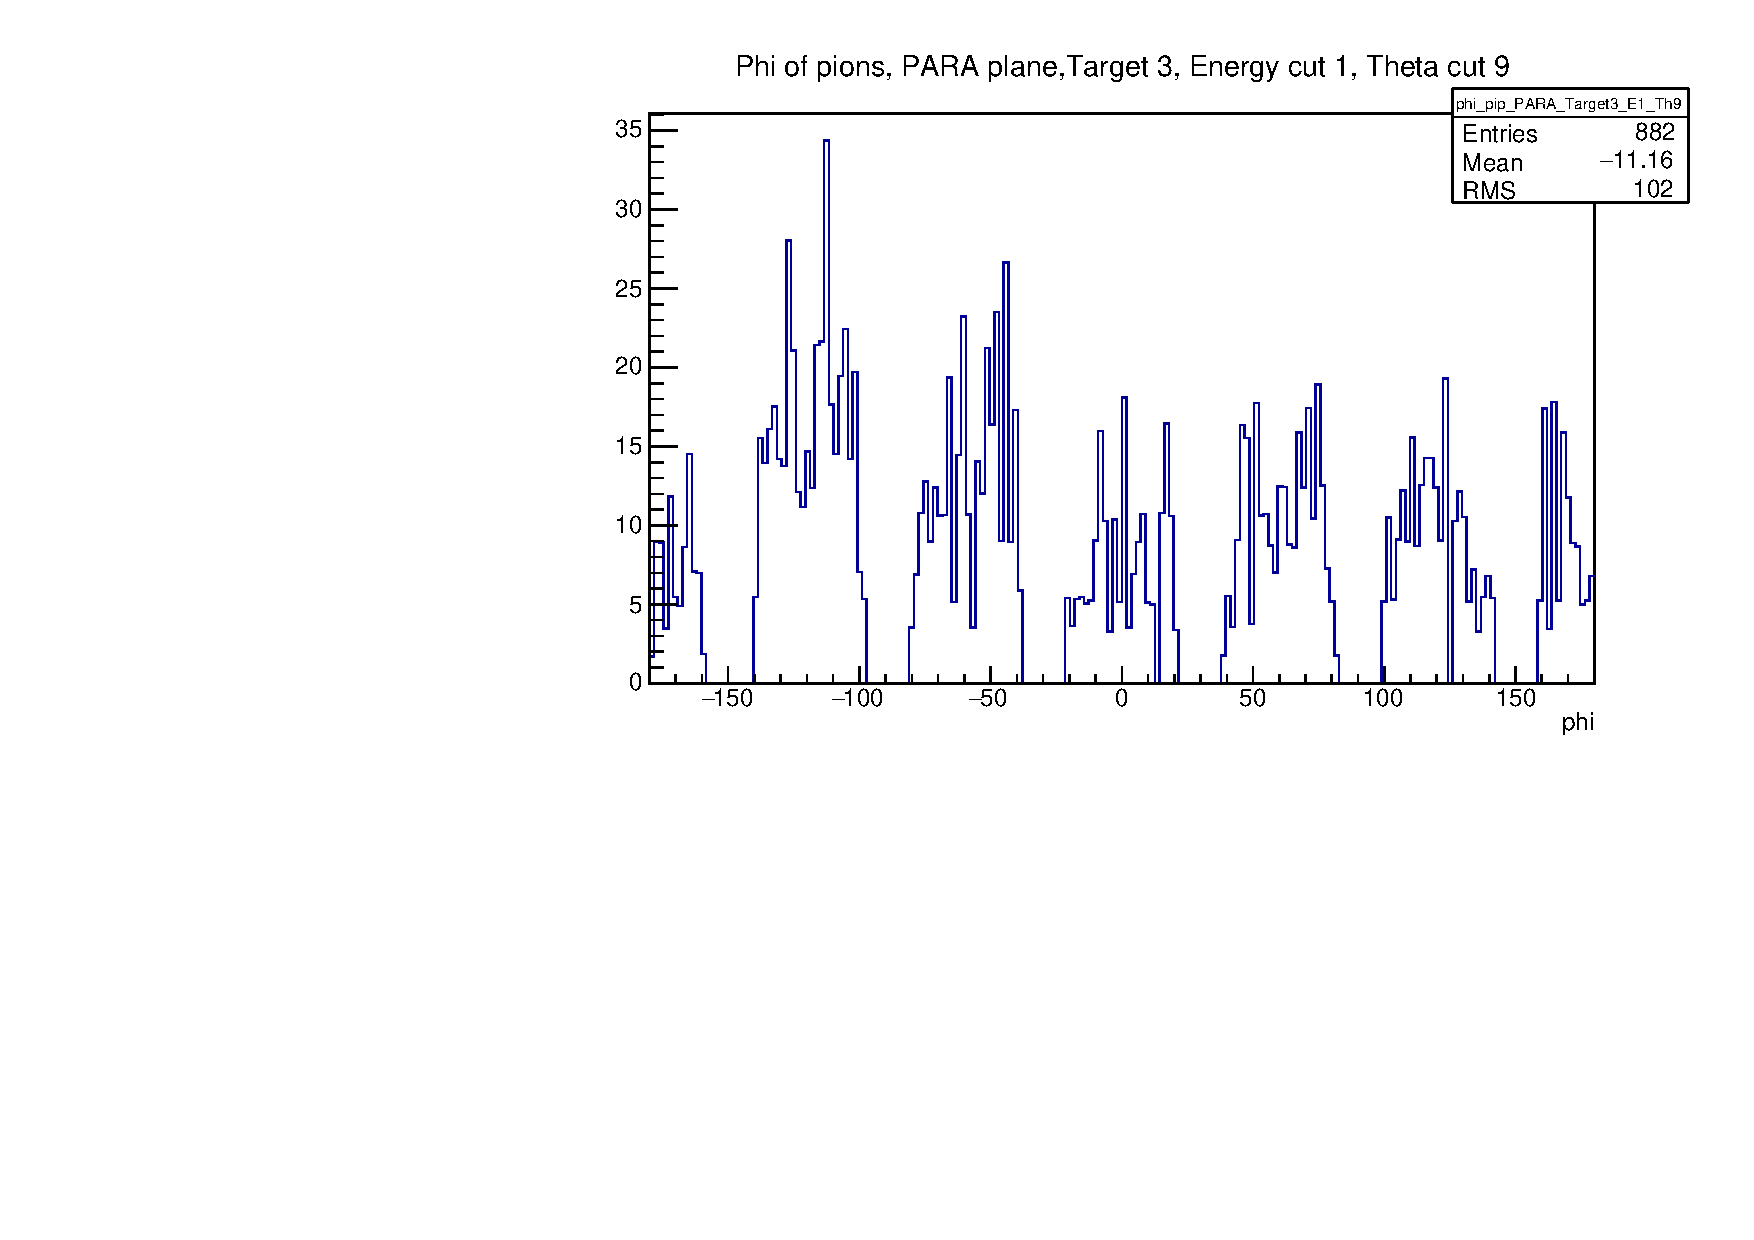
\includegraphics[width=0.6\textwidth]{figures/phi_PARA.pdf} \\
    \caption{$\phi$ distribution for PARA events for a single energy bin and $cos(\theta_{CM})$ bin. }
    \label{fig:frost_PARA_ex}
  \end{center}
\end{figure}



The PARA and PERP $\pi^+$ distributions for a particular target setting were first divided through by the AMO data to remove acceptance effects.
Considering now as:
\begin{itemize}
\item F is the flux on target for each beam setting, which is dependent on both energy and linear beam polarisation. 
\item $\phi_0$ is the “phi-offset” which accounts for any small mis-alignment of the diamond resulting in the beam polarisations not being exactly parallel or exactly perpendicular to the floor.
\end{itemize}

\begin{eqnarray}
N_{\parallel +} = \frac{F_{\parallel}}{F_{AMO}} \left( 1 + P_{\gamma \parallel}cos(2(\phi-\phi_0)) + P_{\gamma \parallel} P_z sin(2(\phi-\phi_0)) \right) \\
N_{\parallel -} = \frac{F_{\parallel}}{F_{AMO}} \left( 1 + P_{\gamma \parallel}cos(2(\phi-\phi_0)) - P_{\gamma \parallel} P_z sin(2(\phi-\phi_0)) \right) \\
N_{\perp +} = \frac{F_{\perp}}{F_{AMO}} \left( 1 + P_{\gamma \perp}cos(2(\phi-\phi_0)) + P_{\gamma \perp} P_z sin(2(\phi-\phi_0)) \right) \\
N_{\perp -} = \frac{F_{\perp}}{F_{AMO}} \left( 1 + P_{\gamma \perp}cos(2(\phi-\phi_0)) - P_{\gamma \perp} P_z sin(2(\phi-\phi_0)) \right) \\
\end{eqnarray}
\begin{figure}[htb]
  \begin{center}
    \subfloat[][Asymmetry for $1.71GeV \leq E_{CM} < 1.74GeV$ and \\$0.4 \leq cos(\theta_{CM}) < 0.6$  ] {
      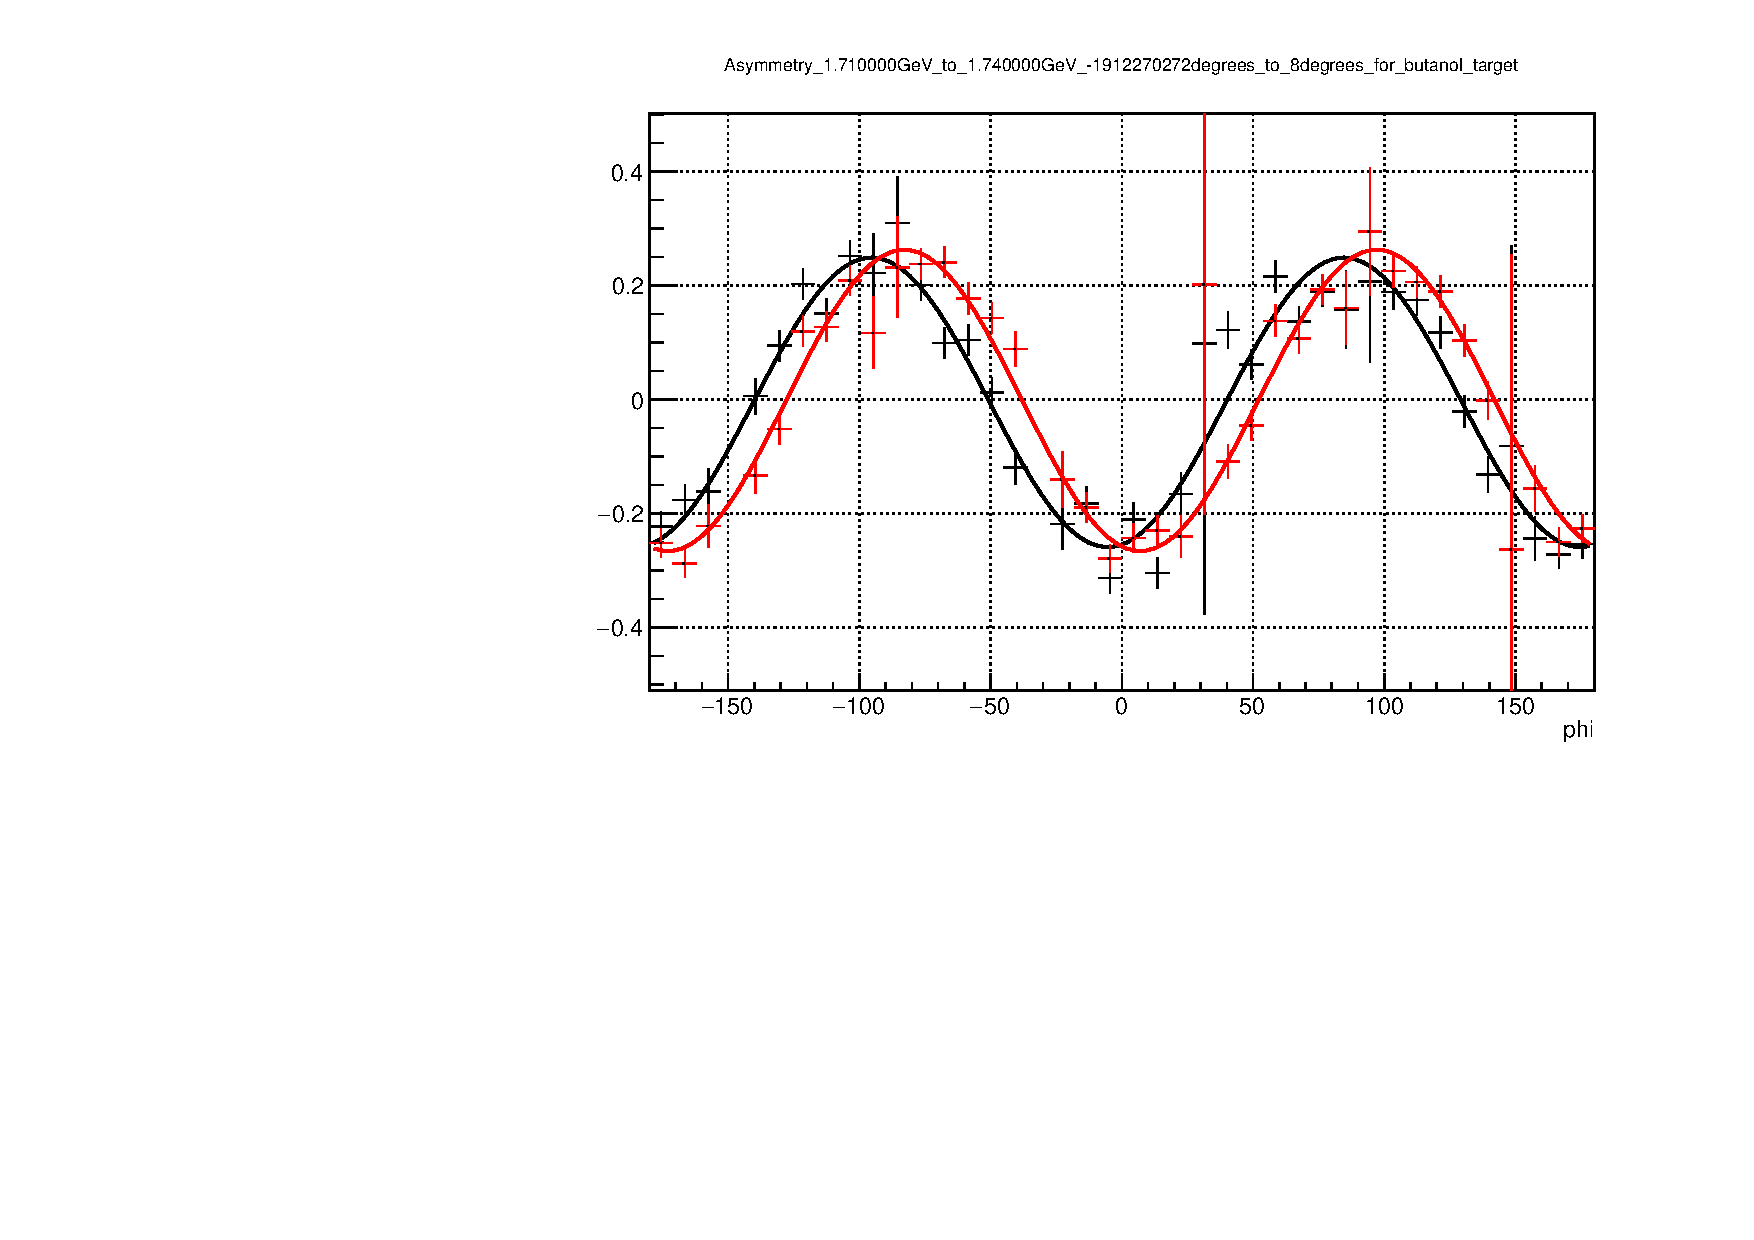
\includegraphics[width=0.5\textwidth]{figures/G_tgpol_effect.pdf} 
      \label{fig:GTgpol_theta1}
    }
    \subfloat[][Asymmetry  $1.54GeV \leq E_{CM} < 1.57GeV$ and \\$-0.6 \leq cos(\theta_{CM}) < -0.4$] {
      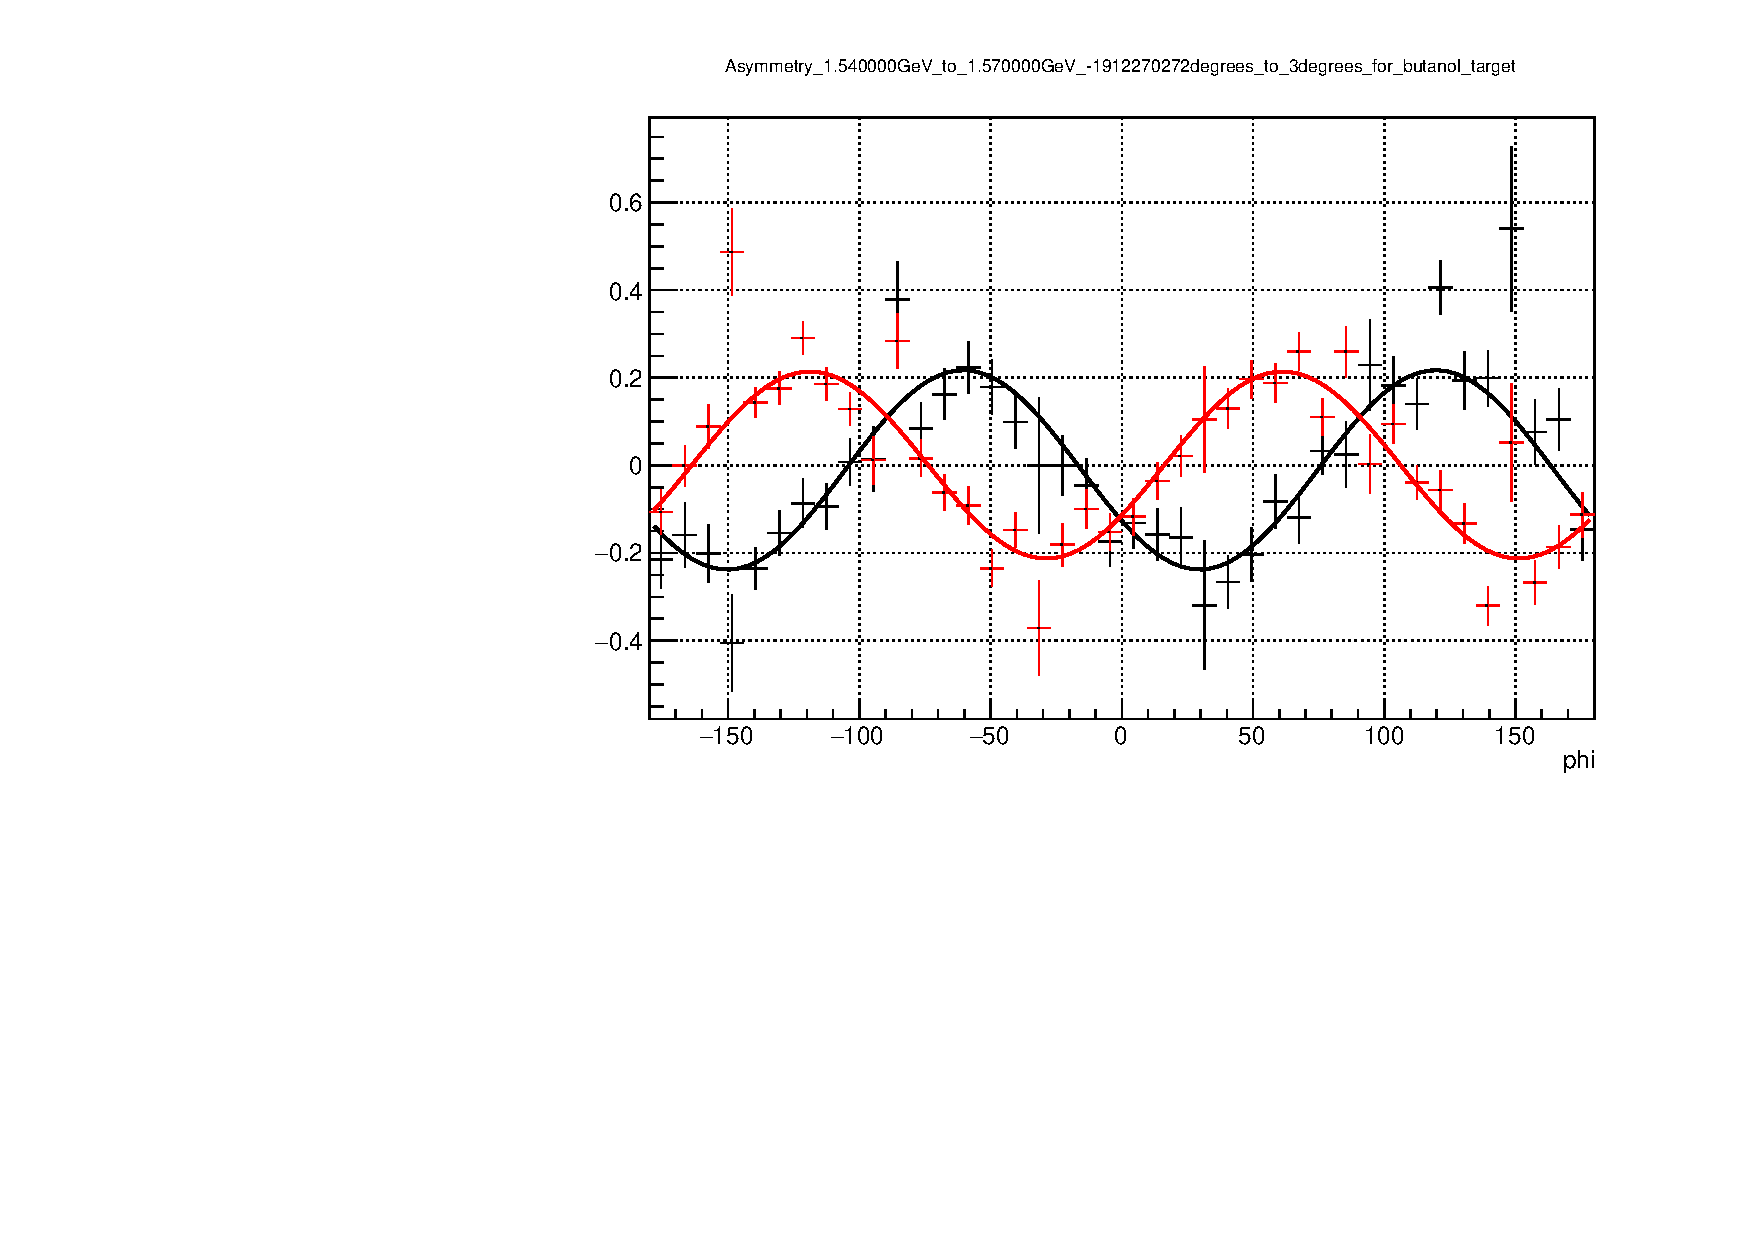
\includegraphics[width=0.5\textwidth]{figures/G_tgpol_effect2.pdf}
    \label{fig:GTgpol_theta2}
    } 
    \caption{The Asymmetry histogram with the fit is plotted for the two different target polarization. One can see the simmetry of the shift from the nominal position in the center ($\phi = 0$).  One can see that, still after the weighting with the Amorphous flux, there is still some effect due to lack of acceptance in the part separating the 6 sectors of CLAS}
  \end{center}
\end{figure}

These distributions where fitted with a function with 4 parameters ($ a,b,c,d $) :
\begin{equation} \label{eqn:fit_flux}
f(\phi) = a \{ 1 + b\, cos[2 (\phi - c) ]  + d\, sin[2(\phi - c)] \} 
\end{equation}
In this fit, $a$ will be directly related to the value that will be use to normalize the PERP and PARA fluxes and $c$ will be a check of the possible $\phi_0$ offset for possible diamond misalignement.
This method of dividing by the amorphous data rather than forming an asymmetry was necessary to allow the PARA and PERP flux to be extracted separately. In order to minimise the statistical error, this calculation was performed for each energy bin. The fit was optimised by calculating first $\phi_0$ and then fixing this value in the fit. 
Using the results of the fits for the PARA ($\parallel$) and PERP ($\perp$) configurations, the ratio between the two different measurements can be determined (using eqn. \ref{eqn:fit_flux}) as:
\begin{equation}
\frac{F_{\perp}}{F_{\parallel}} = \frac{a_{\perp}}{a_{\parallel}}
\end{equation}

\subsection{Calculation of Dilution Factor}
The dilution factor was calculated for each energy and for each $cos(\theta_{CM}$ bin using data obtained from the carbon target to model the unpolarised nucleon background in the butanol target.
As the four vectors of the incident photon, target proton and outgoing pion were known, the neutron four-vector was reconstructed using the missing mass technique:
$$
\gamma \, + \,  p \, \rightarrow \, \pi^+ \, + \, X
$$
\begin{figure}[htb]
  \begin{center}
    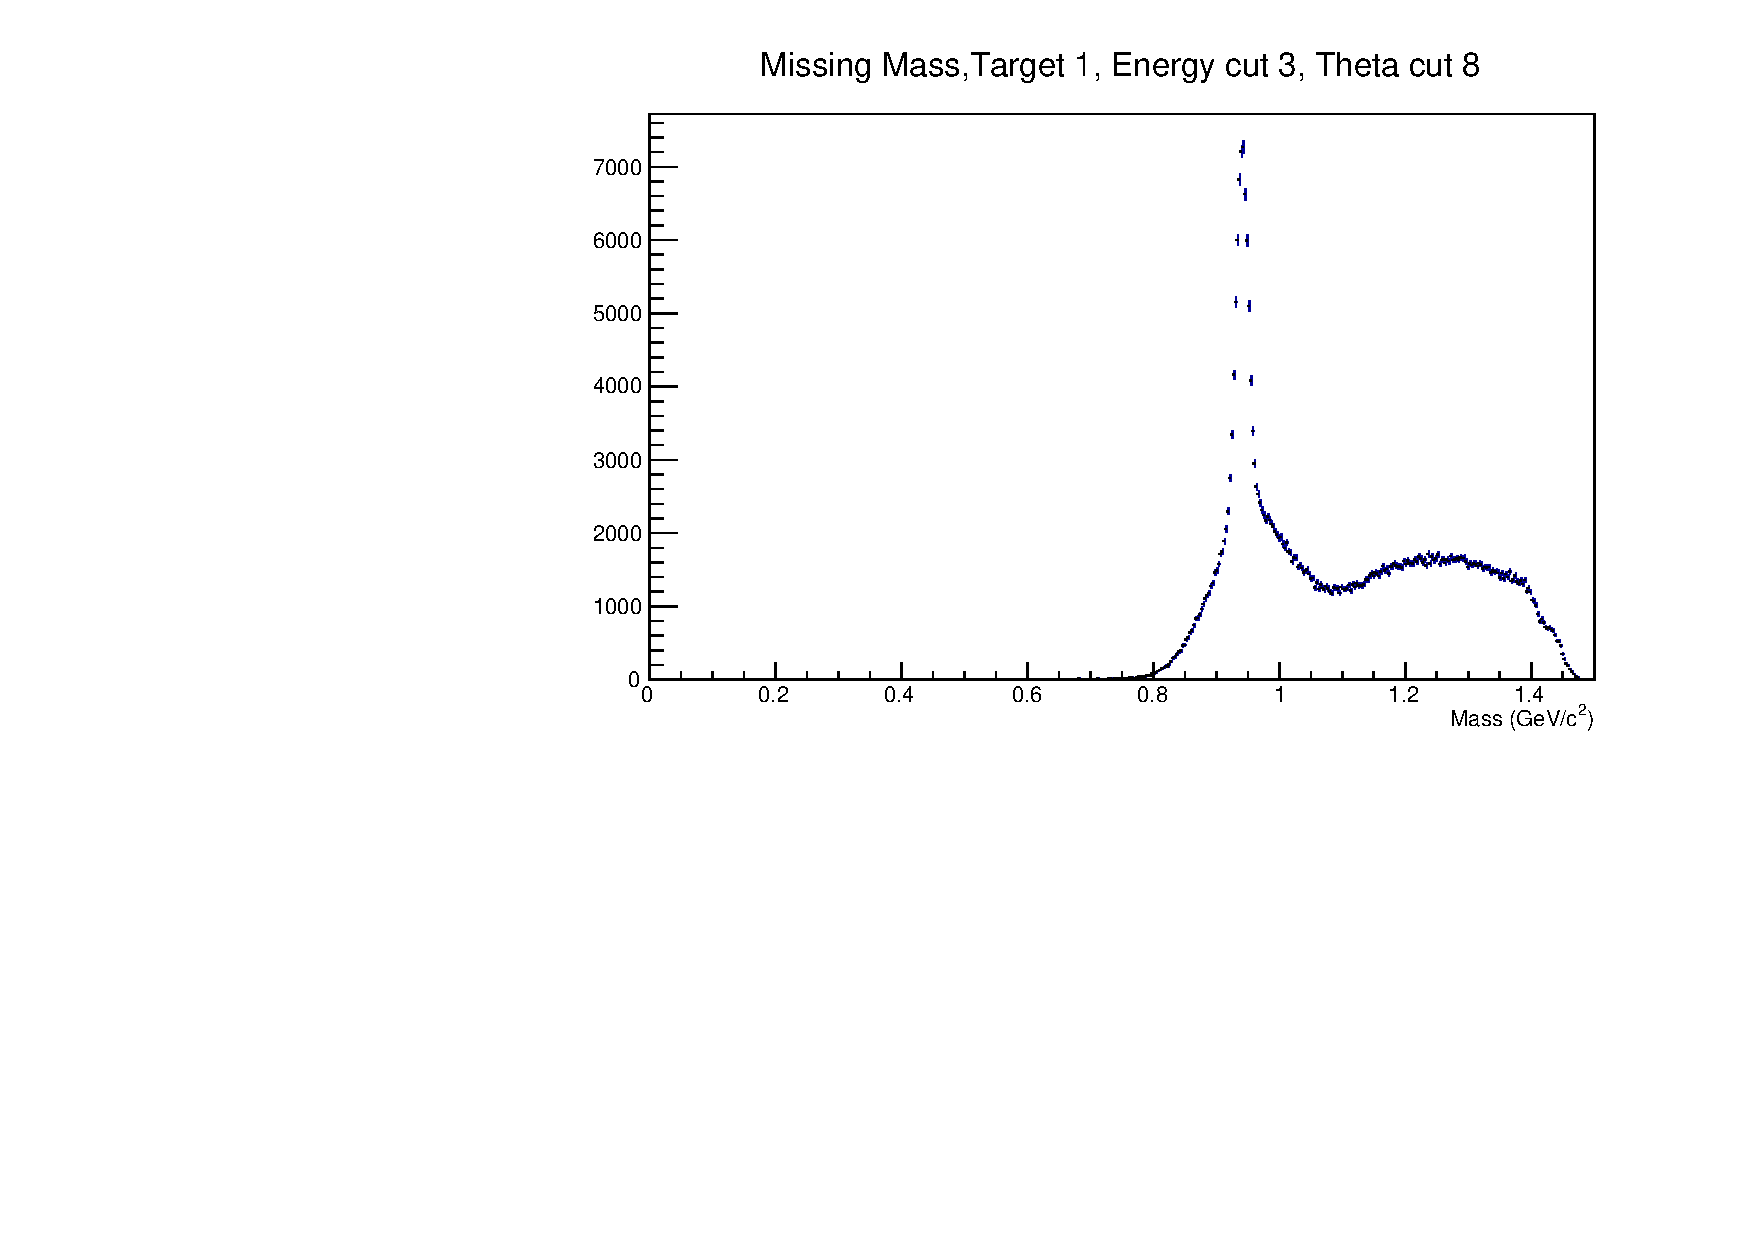
\includegraphics[width=0.6\textwidth]{figures/neutron_missingmass.pdf} \\
    \caption{Mass distribution obtained from the reconstructed neutron four-vector, showing a sharp peak corresponding to the reconstructed neutron and
a broad peak to the right of this corresponding mainly to two-pion production channels. }
    \label{fig:frost_neutronmissing_ex}
  \end{center}
\end{figure}
assuming momentum is conserved in this reaction. Here X can represent the neutron, other neutral particles, or combinations of positively and negatively charged particles such as $\pi^+ , \pi^-$. Figure --- shows the missing mass distribution obtained from the reconstructed neutral four-vector, showing a sharp peak corresponding to the missing neutron mass and a broad peak to the right of this corresponding to other possible channels such as multi-pion production. This plot also shows background contributions due to photon interactions with the carbon and oxygen atoms in the butanol target.
A mass cut was performed to select the neutron and hence the $\pi + n$ events of interest. The width of the neutron-mass squared cut was determined by making a rough subtraction of the carbon and oxygen background using the missing mass distribution obtained from the carbon target data. The missing-mass squared distribution obtained from the carbon target was first scaled to the butanol missing-mass distribution. To obtain the scale factor, the butanol missing mass spectrum was divided by the carbon missing mass spectrum and fit with a Gaussian function in the region of the neutron peak and a zeroth order polynomial in the region to the left of this peak as shown in Figure ---.
As the carbon and butanol targets were very close together in the beamline and could not be fully resolved in the z-vertex distribution spectrum, some events within the carbon z-vertex cuts will have originated from polarised protons within the butanol target.
The carbon missing-mass distribution shown in Figure --- was therefore fit with a combination of two Gaussian functions and a third order polynomial in order to model its shape as shown in Figure ---. One Gaussian function modelled the hydrogen “contamination”, the position and width being taken from the Gaussian fit to the carbon-subtracted butanol missing-mass distribution. The second Gaussian function represented the neutron peak due to the photon interaction with the carbon and oxygen nuclei. Neutron events originating from the photon interaction with a carbon or oxygen nucleus in butanol would be expected to form a peak similar in shape to the neutron peak corresponding to events from the hydrogen atom, but broadened due to the Fermi motion of the nucleons in the carbon or oxygen nucleus. The polynomial modelled the broad background coming from mostly multi-pion production and other non quasi-free processes.
Figure --- shows the butanol missing-mass distribution overlaid with a function representing only the quasi-free background in butanol, and so including only the Gaussian corresponding to events on carbon nuclei and the third order polynomial function obtained from the fit in Figure ---.
At higher energies ($W\geq 1800 MeV$) and more backward angles ($cos(\theta_{CM}) \leq 0$), it was difficult to distinguish either a free or a quasi-free neutron peak in the carbon missing-mass distributions. This effect is due to the relatively small single- pion production cross-section in this kinematical region compared to multi-pion production. An example of such a distribution is shown in Figure ---. In these cases, it was found that a simple third order polynomial fit was more appropriate.
The choice of fit to the carbon missing-mass distributions was determined by comparing the $\chi^2$ per degree of freedom obtained from the two Gaussian plus third order polynomial fit and the simple third order polynomial fit.
The integral of the butanol spectrum and the carbon function within the neutron mass cuts  were then obtained, allowing the dilution factor to be calculated as:
$$
f = \frac{N_B - N_C}{N_B}
$$
where $N_B$ is the integral of the butanol spectrum within the neutron-mass cuts and $N_C$ is the integral of the carbon function within the neutron missing-mass cuts. In order to maximise the statistics available to obtain each data point, it was decided to measure the dilution factor for all W bins, but with the data divided into five $cos(\theta_{CM})$ bins. Graphs of f as a function of $cos(\theta_{CM})$ for each energy bin were fit with a first order polynomial from which the dilution factor for each $cos(\theta_{CM})$  bin could be extracted.
 
